\documentclass{beamer}
\usetheme{Luebeck}
%\usecolortheme{seahorse}
\useinnertheme{rectangles}
\useoutertheme{infolines}
\usepackage{xcolor}
\usepackage[utf8]{inputenc}
\usepackage{tikz}
\usepackage{tabularx}
\usepackage{amsmath,graphicx}
\usetikzlibrary{shapes,backgrounds,arrows,automata,snakes,shadows,positioning, mindmap}
%===================================
\makeatletter
\setbeamertemplate{footline}
{
  \leavevmode%
  \hbox{%
  \begin{beamercolorbox}[wd=.333333\paperwidth,ht=2.25ex,dp=1ex,center]{author in head/foot}%
    \usebeamerfont{author in head/foot}\insertshortauthor%~~\beamer@ifempty{\insertshortinstitute}{}{(\insertshortinstitute)}
  \end{beamercolorbox}%
  \begin{beamercolorbox}[wd=.333333\paperwidth,ht=2.25ex,dp=1ex,center]{title in head/foot}%
    \usebeamerfont{title in head/foot}\insertshorttitle
  \end{beamercolorbox}%
  \begin{beamercolorbox}[wd=.333333\paperwidth,ht=2.25ex,dp=1ex,right]{date in head/foot}%
    \usebeamerfont{date in head/foot}\insertshortdate{}\hspace*{2em}
    \insertframenumber{} / \inserttotalframenumber\hspace*{2ex} 
  \end{beamercolorbox}}%
  \vskip0pt%
}
\makeatother
%===================================
\definecolor{Framableu}{RGB}{12,91,122}
\definecolor{Framableulight}{RGB}{18,144,176}
\definecolor{Nicered}{RGB}{176,18,65}
\definecolor{Lightpink}{RGB}{229,177,218}
\definecolor{Green}{RGB}{144,176,18}
\definecolor{Lightcomplement}{RGB}{235,204,196}
\definecolor{Darkgoldenrod}{RGB}{176,144,18}
\definecolor{Darkomplement}{RGB}{122,43,12}
\definecolor{Complement}{RGB}{176,50,18}
%===================================
\setbeamertemplate{itemize items}[square]
\setbeamertemplate{blocks}[rounded][shadow=false]
\setbeamertemplate{caption}{\raggedright\insertcaption\par}
%===================================
\setbeamercolor{section in head/foot}{fg=white,bg=Framableu}
\setbeamercolor{subsection in head/foot}{fg=white,bg=Framableulight}
\setbeamercolor{author in head/foot}{bg=Framableu}
\setbeamercolor{item}{fg=Framableulight}
\setbeamercolor*{structure}{bg=Framableulight!20,fg=Framableulight}
\setbeamercolor*{palette secondary}{use=structure,fg=white,bg=structure.fg!75}
\setbeamercolor{section in toc}{fg=Framableu,bg=white}
\setbeamercolor{frametitle}{fg=Framableu!80,bg=white}
\setbeamercolor{block title}{fg=white, bg=Framableulight}  
%===================================
\title{Mixture tree model for network inference}
 \subtitle{JOBIM}
\author{Raphaëlle Momal} 
\institute{UMR518 AgroParis Tech/INRA}
\newcommand{\Ccal}{\mathcal{C}}
\newcommand{\edgeunit}{1.5}
\newcommand{\emphase}[1]{\textcolor{Complement}{#1}}
\newcommand\independent{\protect\mathpalette{\protect\independenT}{\perp}}\def\independenT#1#2{\mathrel{\rlap{$#1#2$}\mkern2mu{#1#2}}}
\newcommand{\Ncal}{\mathcal{N}}
\tikzset{%
    observed/.style={%
    scale=0.6,circle,draw=Framableulight,transform shape,fill=white,font=\Large}
}
%#################################################################
\usepackage{graphicx}
\begin{document}
%\AtBeginSection[]{
%   \begin{frame}
   %%% affiche en début de chaque section, les noms de sections et
   %%% noms de sous-sections de la section en cours.
%   \tableofcontents[currentsection,hideothersubsections]
%   \end{frame} 
%}
\frame{\titlepage}


\section{Motivation}
%====================================================================
%====================================================================

\begin{frame}{Context}

Rising interest in \emphase{jointly analysed }species abundances:
\begin{itemize}
	\item Metagenomics 
	\item Microbiologie
	\item Ecology
\end{itemize}
%\pause

\begin{block}{Ecological network}
Tool to better understand species interactions (direct/indirect, nature), eco-systems organizations (clusters ?) 
\end{block}
%\pause
Allows for resilience analyses, pathogens control, ecosystem comparison, reaction prediction...
\end{frame}
%====================================================================
%====================================================================


\begin{frame}{Data}
	\begin{itemize}
	\item \emphase{Species} : animal, bacteria, gene ...
	\item \emphase{Abundances} : ecological counts, Next-Generation Sequencing technologies...
	\item \emphase{Covariates} : coverage, temperature, water depth ... 
\end{itemize}
	Repeated signal : $n$ samples of $p$ abundances.
%\pause
\begin{block}{Notations}
	$Y = [Y_{ij}]_{(i,j) \in \{1,...,n\} \times \{1,..., p\}} $
	\begin{itemize}
	\item $Y_{ij}$ : abundance of the $j^{th}$ species in the $i^{th}$ sample
\end{itemize}
\end{block}
\begin{center}
	\color{Nicered}{Infer the species interaction network from $Y$}
\end{center}
\end{frame}
%====================================================================
%====================================================================
\begin{frame}{Challenges}
	\begin{enumerate}
	\item  Huge space of possible graphs
	\item Count data
	\item Covariables
\end{enumerate}
\end{frame}
%====================================================================
%====================================================================

\section{Network inference}
\subsection{General Framework}
%====================================================================
%====================================================================

\begin{frame}{Graphical models}
	
\begin{columns}
\begin{column}{0.4\linewidth}
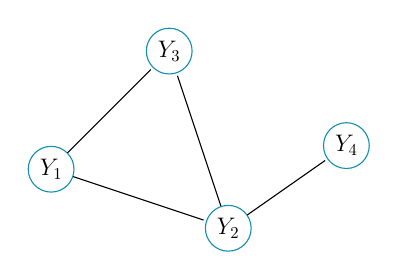
\begin{tikzpicture}	

      \tikzstyle{every edge}=[-,>=stealth',shorten >=1pt,auto,thin,draw]
		\node[observed] (Y1) at (0*\edgeunit, 0*\edgeunit) {$Y_1$};
		\node[observed] (Y2) at (1.5*\edgeunit, -0.5*\edgeunit) {$Y_2$};
		\node[observed] (Y3) at (1*\edgeunit, 1*\edgeunit) {$Y_3$};
		\node[observed] (Y4) at (2.5*\edgeunit, 0.2*\edgeunit) {$Y_4$};
		\path (Y1) edge [] (Y2)
        (Y1) edge [] (Y3)
        (Y2) edge [] (Y3)
        (Y2) edge [] (Y4);
	\end{tikzpicture}\\
\end{column}
\begin{column}{0.6\linewidth}
	\begin{itemize}
	\item All variables are dependant \bigskip
	\item Some are \emphase{conditionnally independant} (i.e. indirectly dependant)\\\bigskip
	 $Y_4$ is independant from $(Y_1, Y_3)$ conditionnally to $Y_2$
\end{itemize}
\end{column}
\end{columns}
\end{frame}
%====================================================================
%====================================================================

\begin{frame}{Graphical models}
\begin{block}{Definition}
	The joint distribution P is faithful to the graph G iff \[ P(Y_1, \dots, Y_p) \propto \prod_{C \in \Ccal_G} \psi_C(Y_C) \]
  where $\Ccal_G =$ set of cliques of $G$.
\end{block}
%\pause
\begin{columns}
\begin{column}{0.4\linewidth}
\flushright
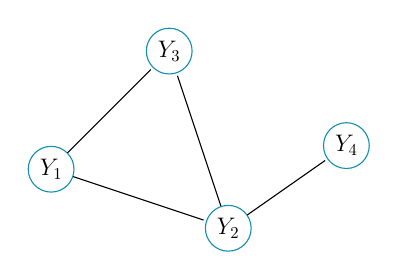
\begin{tikzpicture}	

      \tikzstyle{every edge}=[-,>=stealth',shorten >=1pt,auto,thin,draw]
		\node[observed] (Y1) at (0*\edgeunit, 0*\edgeunit) {$Y_1$};
		\node[observed] (Y2) at (1.5*\edgeunit, -0.5*\edgeunit) {$Y_2$};
		\node[observed] (Y3) at (1*\edgeunit, 1*\edgeunit) {$Y_3$};
		\node[observed] (Y4) at (2.5*\edgeunit, 0.2*\edgeunit) {$Y_4$};
		\path (Y1) edge [] (Y2)
        (Y1) edge [] (Y3)
        (Y2) edge [] (Y3)
        (Y2) edge [] (Y4);
	\end{tikzpicture}\\
\end{column}
\begin{column}{0.6\linewidth}
\begin{align*}
	P(Y_1, &Y_2, Y_3, Y_4) \propto \\ 
	& \psi_1(Y_1 ,Y_2, Y_3) \times \psi_2(Y_3, Y_4)
\end{align*} 
\end{column}
\end{columns}
\end{frame}

\subsection{Using trees}
%====================================================================
%====================================================================

\begin{frame}{Spanning trees}
	
  \begin{columns}
  \begin{column}{6cm}Much \emphase{ smaller space} to explore:\\ $\text{\#} \mathcal{G} = 2^{\frac{p(p-1)}{2}}$ vs. $\text{\#} \mathcal{T} = p^{(p-2)}$
	
	\end{column}
	 \begin{column}{6cm}
	\begin{figure}[htp]
\includegraphics[width=5cm]{compar_typegraphs.png}
	\end{figure}
\end{column}
\end{columns}
Spanning trees are a \emphase{sparse} solution :
	$$
  \left. \begin{tabular}{l}
          $G$ is connected \\
          $G$ has no cycle
         \end{tabular} \right\}
  \text{ $G$ has $(p-1)$ edges}
  $$

\end{frame}
%====================================================================
%====================================================================
\begin{frame}{Complexity}
	
\end{frame}
%====================================================================
%====================================================================

\begin{frame}{Tree averaging} 

\begin{tabular}{p{.4\textwidth}}
 \begin{tabular}{ccccl}
   \begin{tabular}{c}
	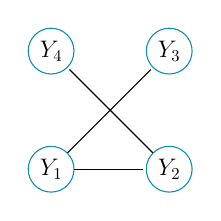
\begin{tikzpicture}
		
      \tikzstyle{every edge}=[-,>=stealth',shorten >=1pt,auto,thin,draw]
    
		\node[observed] (Y1) at (0*\edgeunit, 0*\edgeunit) {$Y_1$};
		\node[observed] (Y2) at (1*\edgeunit, 0*\edgeunit) {$Y_2$};
		\node[observed] (Y3) at (1*\edgeunit, 1*\edgeunit) {$Y_3$};
		\node[observed] (Y4) at (0*\edgeunit, 1*\edgeunit) {$Y_4$};
		\path (Y1) edge [] (Y2)
        (Y1) edge [] (Y3)
        (Y2) edge [] (Y4);
   
	\end{tikzpicture}\\
	\footnotesize{$P\{T = T_1 | Y\}$}
	   \end{tabular}
	   & 
	   \hspace{-.05\textwidth}% \pause
	   \begin{tabular}{c}
		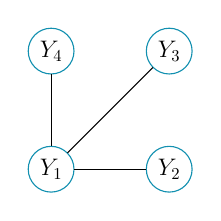
\begin{tikzpicture}
		\tikzstyle{every observed}=[draw=none,text=black,scale=0.5,
      transform shape,circular drop shadow] 
		\node[observed] (Y1) at (0*\edgeunit, 0*\edgeunit) {$Y_1$};
		\node[observed] (Y2) at (1*\edgeunit, 0*\edgeunit) {$Y_2$};
		\node[observed] (Y3) at (1*\edgeunit, 1*\edgeunit) {$Y_3$};
		\node[observed] (Y4) at (0*\edgeunit, 1*\edgeunit) {$Y_4$};
		
		\path (Y1) edge [] (Y2)
        (Y1) edge [] (Y3)
        (Y1) edge [] (Y4);
		\end{tikzpicture} \\
		\footnotesize{$P\{T = T_2 | Y\}$}
	   \end{tabular}
	   &
	   \hspace{-.05\textwidth} %\pause
	   \begin{tabular}{c}
		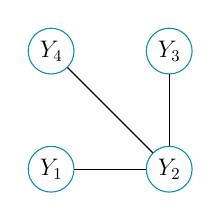
\begin{tikzpicture}
		\tikzstyle{every observed}=[draw=none,text=black,scale=0.5,
      transform shape,circular drop shadow] 
		\node[observed] (Y1) at (0*\edgeunit, 0*\edgeunit) {$Y_1$};
		\node[observed] (Y2) at (1*\edgeunit, 0*\edgeunit) {$Y_2$};
		\node[observed] (Y3) at (1*\edgeunit, 1*\edgeunit) {$Y_3$};
		\node[observed] (Y4) at (0*\edgeunit, 1*\edgeunit) {$Y_4$};
		
		\path (Y1) edge [] (Y2)
        (Y2) edge [] (Y3)
        (Y2) edge [] (Y4); 
		\end{tikzpicture}\\
		\footnotesize{$P\{T = T_3 | Y\}$}
	   \end{tabular}
	   &
	   \hspace{-.05\textwidth}% \pause
	   \begin{tabular}{c}
		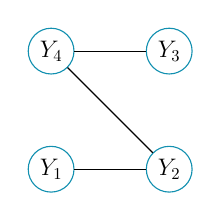
\begin{tikzpicture}
		\tikzstyle{every observed}=[draw=none,text=black,scale=0.5,
      transform shape,circular drop shadow] 
		\node[observed] (Y1) at (0*\edgeunit, 0*\edgeunit) {$Y_1$};
		\node[observed] (Y2) at (1*\edgeunit, 0*\edgeunit) {$Y_2$};
		\node[observed] (Y3) at (1*\edgeunit, 1*\edgeunit) {$Y_3$};
		\node[observed] (Y4) at (0*\edgeunit, 1*\edgeunit) {$Y_4$};
		 
		\path (Y1) edge [] (Y2)
        (Y3) edge [] (Y4)
        (Y2) edge [] (Y4);
		\end{tikzpicture} \\
		\footnotesize{$P\{T = T_4 | Y\}$}
	   \end{tabular}
	   & \hspace{-.06\textwidth} \huge{\emphase{...}}\normalsize   \\ \\
	   \\% \pause
	   \begin{tabular}{l}
		Compute edge\\
		probabilities:
	   \end{tabular}
	   &
	   \hspace{-.05\textwidth}
	   \begin{tabular}{c}
		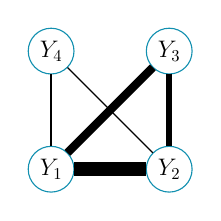
\begin{tikzpicture}
		\node[observed] (Y1) at (0*\edgeunit, 0*\edgeunit) {$Y_1$};
		\node[observed] (Y2) at (1*\edgeunit, 0*\edgeunit) {$Y_2$};
		\node[observed] (Y3) at (1*\edgeunit, 1*\edgeunit) {$Y_3$};
		\node[observed] (Y4) at (0*\edgeunit, 1*\edgeunit) {$Y_4$};
		\draw [line width=5pt] (Y1) -- (Y2); 
		\draw [line width=3pt] (Y1) -- (Y3); 
		\draw [line width=.5pt] (Y1) -- (Y4); 
		\draw [line width=2pt] (Y2) -- (Y3); 
		\draw [line width=.5pt] (Y2) -- (Y4); 
 %		\draw [line width=.5pt] (Y3) -- (Y4); 
		\end{tikzpicture}\\
		\emphase{$P\{(j, k) \in T | Y\}$}
	   \end{tabular}
	   &
	   \hspace{-.05\textwidth} %\pause
	   \begin{tabular}{l}
		Thresholding\\
		probabilities:
	   \end{tabular}
	   &
	   \hspace{-.05\textwidth}
	   \begin{tabular}{c}
		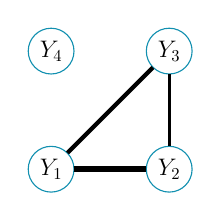
\begin{tikzpicture}
		\node[observed] (Y1) at (0*\edgeunit, 0*\edgeunit) {$Y_1$};
		\node[observed] (Y2) at (1*\edgeunit, 0*\edgeunit) {$Y_2$};
		\node[observed] (Y3) at (1*\edgeunit, 1*\edgeunit) {$Y_3$};
		\node[observed] (Y4) at (0*\edgeunit, 1*\edgeunit) {$Y_4$};
		\draw [line width=2pt] (Y1) -- (Y2); 
		\draw [line width=1.5pt] (Y1) -- (Y3); 
% 		\draw [line width=1pt] (Y1) -- (Y4); 
		\draw [line width=1pt] (Y2) -- (Y3); 
% 		\draw [line width=.1pt] (Y2) -- (Y4); 
% 		\draw [line width=1pt] (Y3) -- (Y4); 
		\end{tikzpicture}\\
		\emphase{$P\{(j, k) \in T | Y\}$}
	   \end{tabular}
	   &
	 \end{tabular}
    \end{tabular}
\end{frame}
%====================================================================
%====================================================================


\section{With count data}
\subsection{Model}

%====================================================================
%====================================================================

\begin{frame}{PLN model}
\begin{block}{Poisson log-Normal distribution}
\[
            \left.
                \begin{array}{rl}
                Z_i \textit{ iid } &\sim \mathcal{N}_{d}(0,\Sigma)\\
                    &(Y_{ij})_j \independent |Z_i\\
                    Y_{ij}|Z_{ij} &\sim \mathcal{P}(e^{\only<2-3>{\emphase{o_{ij}+x_i^{\text{T}}\Theta_j} +}Z_{ij}}) 
                   
                \end{array}
            \right \} Y \sim \mathcal{PLN}(\only<2-3>{\emphase{O+x^{\text{T}}\Theta }}\only<1>{0}, \Sigma)  
            \]
\end{block}
\vspace{0.5cm}
\begin{itemize}
    \item Gaussian latent layer
    \item Easy handling of multi-variate data (contrary to Negative binomial distribution)
  \only<2-3>{ \item Allow adjustment for covariates and offsets}
\end{itemize}
%\pause
\only<3>{\center{ \textbf{ Idea:} Infer the \emphase{latent Gaussian network.}}}
\end{frame}

%====================================================================
%====================================================================
\section{Simulation}
\subsection{Competitor}
%====================================================================
%====================================================================

\begin{frame}{Gaussian Graphical Models (GGM) \& SpiecEasi}
   \emphase{Gaussian distribution.}\\
 \begin{center}
	$  Y_r \sim \Ncal_p(\mu, \Sigma) $, $\mu =$ vector of means, $\Sigma =$ covariance matrix.
 % \[L(Y,\Omega) \propto \frac{n}{2}\log(det(\Omega))-\frac{n}{2} Y^T\Omega Y\]
\end{center}
  
 
  
   \bigskip %\pause
  \emphase{A nice property.} ~ \\

  \begin{columns}
  \begin{column}{0.05\textwidth}
	
\end{column}
  \begin{column}{0.4\textwidth}
   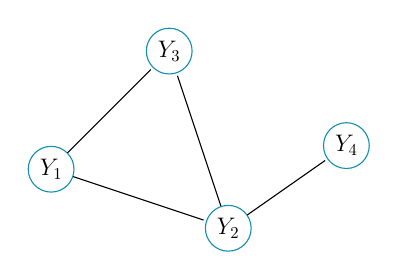
\begin{tikzpicture}	

       \tikzstyle{every edge}=[-,>=stealth',shorten >=1pt,auto,thin,draw]
		\node[observed] (Y1) at (0*\edgeunit, 0*\edgeunit) {$Y_1$};
		\node[observed] (Y2) at (1.5*\edgeunit, -0.5*\edgeunit) {$Y_2$};
		\node[observed] (Y3) at (1*\edgeunit, 1*\edgeunit) {$Y_3$};
		\node[observed] (Y4) at (2.5*\edgeunit, 0.2*\edgeunit) {$Y_4$};
		\path (Y1) edge [] (Y2)
        (Y1) edge [] (Y3)
        (Y2) edge [] (Y3)
        (Y2) edge [] (Y4);
	\end{tikzpicture}
    \end{column}
    \begin{column}{12cm}
    \begin{tabular}{p{.5\textwidth}}
	 Inverse covariance matrix
	 $$
	 \Sigma^{-1} = \Omega \propto \left[ \begin{array}{cccc}
	   1 & .5 & .5 & \emphase{0} \\
	   .5 & 1 & .5 & \emphase{0} \\
	   .5 & .5 & 1 & .5 \\
	   \emphase{0} & \emphase{0} & .5 & 1
	   \end{array} \right] 
	 $$
    \end{tabular} 
   
  \end{column}
  \end{columns}
 \emphase{Glasso.}\\\bigskip
 On gaussian data : $\widehat{\Omega}_\lambda = \arg\min_{\Omega \in \mathcal{S}_d^+}\left\{ L(Y,\Omega)+\lambda \sum_{i\neq j} |\omega_{ij}| \right\} \hspace{0.5cm} $\\
 \begin{center}
	$\Rightarrow$ {\color{Nicered}SpiecEasi method} with centered log-ratio transformation of count data.
\end{center}

% $$
% \widehat{\Sigma} \propto \left[ \begin{array}{cccc}
%   1 & -.02 & -.49 & .25 \\
%   -.02 & 1 & -.62 & .36 \\
%   -.49 & -.62 & 1 & -.61 \\
%   .25 & .36 & -.61 & 1
%   \end{array} \right] 
% $$

\end{frame}
%====================================================================
%====================================================================

\subsection{}
%====================================================================
%====================================================================

\begin{frame}{Simulation agenda}
\begin{enumerate}
     \item Draw $G$ \vspace{0.3cm}
     \item Derive $\Omega$  from the adjacency matrix\vspace{0.3cm} 
     \item Generate count data $Y$ under PLN model with parameter $\Omega$ and possible covariates
     \item Infer{\fontfamily{qcr}\selectfont
PLNmodels} : ajuster le modèle de régression PLN à partir de $\Sigma_Z$, $\Rightarrow \hat{\Sigma}_Z$\vspace{0.3cm}
   
     \item Appliquer le glasso et notre EM à $\hat{\Sigma}_Z$\vspace{0.3cm}
     \item Comparer les graphes obtenus et G
 \end{enumerate}

	
\end{frame}
%====================================================================
%====================================================================

\begin{frame}{Results}
	\begin{figure}[htp]
\centering
\includegraphics[scale=0.6]{erdos_d.pdf}
\caption{}
\label{}
\end{figure}

\end{frame}


%====================================================================
%====================================================================
\section{Application}
\subsection{Oak data}

%====================================================================
%====================================================================

\begin{frame}{Oak Mildew}
\begin{columns}
\begin{column}{5cm}
\begin{figure}[htp]
\centering
\includegraphics[scale=0.07]{EA.jpg}
\caption{\textit{Erysiphe alphitoides.}}
\end{figure}
\end{column}
\begin{column}{6cm}
\begin{figure}[htp]
\centering
\includegraphics[scale=0.1]{mildew.jpg}
\caption{Oak leaf with powdery mildew.}
\end{figure}
\end{column}
\end{columns}
\vspace{0.5cm}
Data : metabarcoding of microbiome on oak tree leaves 
\begin{itemize}
	\item 114 sample of 94 microbial species counts (bacteria/fungi)
	\item Offsets for each sample and specific for bacteria and fungi
	\item 4 covariables : 3 distances (quantitative), 1 orientation (qualitative)
\end{itemize}
\end{frame}
%====================================================================
%====================================================================

\begin{frame}{Results}

\begin{columns}
\begin{column}{0.5\linewidth}
\begin{figure}[H]
\caption{Offset only}
\includegraphics[width=6cm]{net1.png}
\end{figure}
\end{column}
\begin{column}{0.5\linewidth}
\begin{figure}[H]
\caption{Offset and distance covariables}
\includegraphics[width=6cm]{netdist.png}
\end{figure}
\end{column}
\end{columns}
\end{frame}
%====================================================================
%====================================================================

\begin{frame}{Perspectives}
We provide : \\
What is next :
	\begin{itemize}
	\item threshold study
	\item Network comparison
	\item Inference in the observe counts layer
	\item Missing major entity (species / covariable)
\end{itemize}
\end{frame}
\end{document}